\chapter{11.7 习题}
\begin{flushleft}
1.证明当 $L_{w}=0$时,一般阴影矩阵$S$缩减为$S_{dir}$,当$L_{w}=1$时,$S$缩减为$S_{point}$\\
2.证明 $s=p-\frac{n\cdot p+d}{n\cdot (p-L)}(p-L)=pS_{point}$,通过对每个分量进行矩阵乘法,如11.5.1中针对定向灯所做的那样。\\
3.修改“镜像”演示,生成图\ref{fig:11-1}中的“左”图像。\\
4.修改“镜像”演示,生成图\ref{fig:11-10}中的“左”图像。\\
5.修改“镜像”演示。首先用下面的深度设置绘制一堵墙:\\
\end{flushleft}

\begin{lstlisting}
depthStencilDesc.DepthEnable = false;
depthStencilDesc.DepthWriteMask = D3D12_DEPTH_WRITE_MASK_ALL;
depthStencilDesc.DepthFunc = D3D12_COMPARISON_LESS;
\end{lstlisting}

\begin{flushleft}
接着,在墙后面用下面深度设置绘制头骨:\\
\end{flushleft}

\begin{lstlisting}
depthStencilDesc.DepthEnable = true;
depthStencilDesc.DepthWriteMask = D3D12_DEPTH_WRITE_MASK_ALL;
depthStencilDesc.DepthFunc = D3D12_COMPARISON_LESS;
\end{lstlisting}

\begin{flushleft}
墙是否遮挡了头骨?请说明原因。如果您使用以下方法来绘制墙壁会发生什么?\\
\end{flushleft}

\begin{lstlisting}
depthStencilDesc.DepthEnable = true;
depthStencilDesc.DepthWriteMask = D3D12_DEPTH_WRITE_MASK_ALL;
depthStencilDesc.DepthFunc = D3D12_COMPARISON_LESS;
\end{lstlisting}

\begin{flushleft}
请注意,此练习不使用模板缓冲区,应在该练习中禁用模板缓冲区。\\

6.修改“镜像”演示,不反转三角形绕线顺序。反射的茶壶是否正确渲染?\\
7.修改第10章中的“Blend”演示,在场景的中心绘制一个圆柱体(没有帽子)。 使用加法混合在本章的目录中找到60帧动画电子螺栓动画来构造圆柱体。效果如图\ref{fig:11-11}。\\
\end{flushleft}

\begin{figure}[h]
    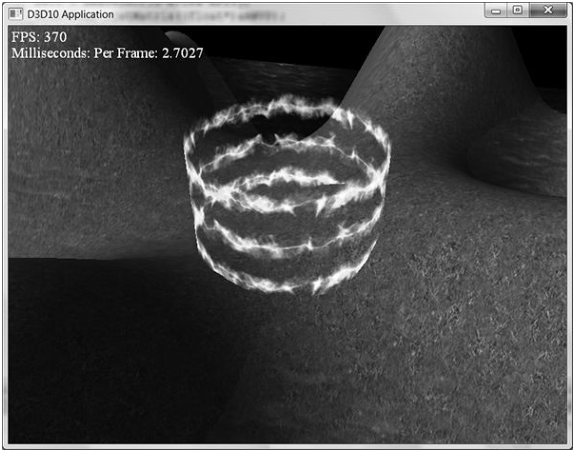
\includegraphics[width=\textwidth]{11-11}
    \centering
    \caption{练习7的效果截图}
    \label{fig:11-11}
\end{figure}

\begin{flushleft}
8.深度复杂度是指通过深度测试竞争写入后缓冲器中的特定条目的像素片段的数量。 例如,我们绘制的像素可能被更接近相机的像素覆盖(并且在绘制整个场景后实际计算出最近的像素之前,这可能会发生几次)。 图\ref{fig:11-12}中的像素的深度复杂度为3,因为三个像素片段竞争像素。
\end{flushleft}

\begin{figure}[h]
    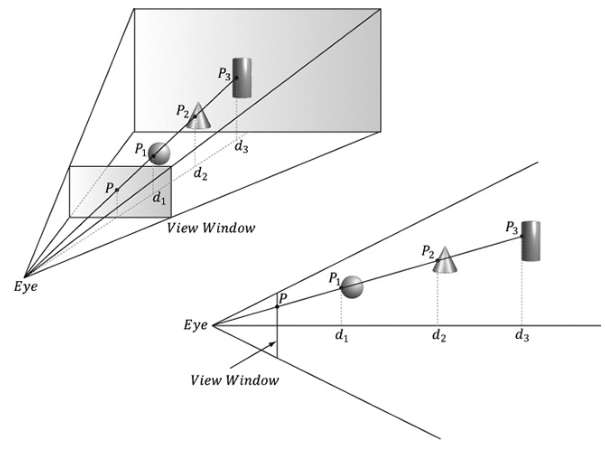
\includegraphics[width=\textwidth]{11-12}
    \centering
    \caption{多个像素片段竞争渲染到投影窗口上的单个像素。在该场景中,像素P的深度复杂度为3。}
    \label{fig:11-12}
\end{figure}

\begin{flushleft}
可能,显卡每帧可以填充几次像素。 这种过度绘制会影响性能,因为显卡浪费时间处理这些像素,最终被覆盖。 所以,测量场景中的深度复杂度以进行性能分析是有用的。\\

我们能以如下方式测量深度复杂度:渲染场景并使用模板缓冲区作为计数器; 也就是说,模板缓冲区中的每个像素最初都被清零,每次处理像素片段时,我们都会用 D3D12\_STENCIL\_OP\_INCR 递增计数。使用模板比较函数 D3D12\_COMPARISON\_ALWAYS,对应的模板缓冲区条目会始终为每个像素片段递增。 然后,例如,在绘制帧之后,如果第$i$个像素在模板缓冲区中具有相应的五个条目,则知道在该帧期间针对该像素处理了五个像素片段(即,像素深度复杂度为五)。 请注意,在计算深度复杂度时,从技术上讲,您只需要将场景渲染到模板缓冲区即可。\\

要可视化深度复杂度(存储在模板缓冲区中),请执行以下操作:\\

1.为每个深度复杂度$k$关联颜色$c_{k}$。 例如,蓝色表示深度复杂度为$1$,绿色表示深度复杂度为$2$,红色表示深度复杂度为$3$,依此类推。 (在非常复杂的场景中,像素的深度复杂度会变得非常大,您可能不希望为每个级别关联一种颜色。相反,您可以将颜色与一段连续的复杂度关联。例如,具有深度的像素复杂度1-5为蓝色,深度复杂度为6-10的像素为绿色,依此类推。)\\

2.将模板缓冲区操作符设置为 D3D12\_STENCIL\_OP\_KEEP,不再修改它。 (当我们在渲染场景,计算深度复杂度时,用 D3D12\_STENCIL\_OP\_INCR 修改模板缓冲区,但是当编写代码来可视化模板缓冲区时,我们只需要从模板缓冲区读取,我们不应该写入它。)\\

3.对于每个深度复杂度$k$级:\\
\end{flushleft}

\begin{itemize}
  \item (1).将模板比较功能设置为 D3D12\_COMPARISON\_EQUAL,并将模板参考值设置为$k$。
  \item (2).绘制覆盖整个投影窗口的四边形颜色$c_{k}$。 请注意,由于前面的模板比较功能和参考值,这只会对深度复杂度为$k$的像素进行着色。
\end{itemize}

\begin{flushleft}
通过这种设置,我们可以根据其深度复杂度对每个像素进行唯一着色,因此我们可以轻松地研究场景的深度复杂性。 在本练习中,渲染第10章“Blend”演示中使用的场景的深度复杂度。图\ref{fig:11-13}显示了一个示例屏幕截图。
\end{flushleft}

\begin{figure}[h]
    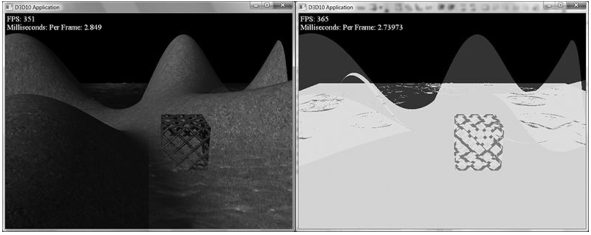
\includegraphics[width=\textwidth]{11-13}
    \centering
    \caption{练习8的截图}
    \label{fig:11-13}
\end{figure}

\begin{flushleft}
~\\
NOTICE:深度测试发生在管道的输出合并阶段,该阶段发生在像素着色器阶段之后。这意味着即使最终可能被深度测试拒绝,也会经过像素着色器处理像素片段。现代硬件会进行“early z-test”,这会在像素着色器之前执行深度测试。这样,被丢弃的像素片段在可能被昂贵的像素着色器处理之前被丢弃。要利用此优化,您应该尝试相对于相机以前后顺序渲染非混合游戏对象;首先绘制最近的对象,它们后面的对象就会无法通过early z-test而不会被进一步处理。如果由于高深度复杂性而导致场景遭受大量过度绘制的情况,使用 early z-test 会带来显着的性能优势。我们无法通过Direct3D API控制early z-test;是否可以执行early z-test由图形驱动程序决定。例如,如果像素着色器会修改像素片段的深度值,则不可能进行early z-test,因为像素着色器必须在深度测试之前执行。
~\\
NOTICE: 我们提到了修改像素着色器中像素深度的功能。这是如何运作的? 像素着色器实际上可以输出结构体,而不仅仅是我们到目前为止所做的单个颜色向量:\\
\end{flushleft}

\begin{lstlisting}
struct PixelOut
{
    float4 color : SV_Target;
    float depth : SV_Depth;
};
PixelOut PS(VertexOut pin)
{
    PixelOut pout;
    // ...usual pixel work
    pout.Color = float4(litColor, alpha);
    // set pixel depth in normalized [0, 1] range
    pout.depth = pin.PosH.z - 0.05f;
    return pout;
}
\end{lstlisting}

\begin{flushleft}
SV\_Position 元素的 z坐标(pin.PosH.z)给出未修改的像素深度值。使用特殊系统值语义 SV\_Depth,像素着色器可以输出修改的深度值。\\
~\\
9.实现深度复杂性可视化的另一种方法是使用加法混合。首先清除后面的缓冲区黑色并禁用深度测试。接下来,将源和目标混合因子都设置为 D3D12\_BLEND\_ONE,将混合操作设置为 D3D12\_BLEND\_OP\_ADD,以使混合方程看起来像 $C=C_{src}+C_{dst}$。观察这个公式,对于每个像素,累加写入它的所有像素片段的颜色。现在使用像素着色器渲染场景中的所有对象,该像素着色器输出低强度颜色,如$(0.05,0.05,0.05)$。一个像素越多的过度绘制,这些低强度颜色累加,增加了亮度。例如,如果一个像素过度绘制了十次,那么它的颜色强度将为$(0.5,0.5,0.5)$。因此,在渲染场景之后每个像素的强度显示了该像素的深度复杂度。使用第10章中的“Blend”演示作为测试场景,实现此版本的深度复杂度测量。\\

10.解释如何计算通过深度测试的像素数。解释如何计算未通过深度测试的像素数?\\
11.修改“镜子”演示,除头骨之外在镜子中对地面做镜面反射。\\
12.从阴影渲染项的世界矩阵中删除垂直偏移量,以便您可以看到 z-fighting 现象。\\
\end{flushleft}
